\chapter{General introduction}
\label{part:intro}


\section{Industrial challenges} 


Sedimentation of particles falling or rising under the action of gravity through a fluid is frequently used in a variety of industrial and natural processes, such as food processing, cosmetics, petroleum production, and environmental remediation. 
It is an efficient way to separate solid particles or droplets from the surrounded fluid. 
The clarification of waste water makes use of such a physics, the particles or droplets rise up due to buoyancy forces, afterward they are ejected from the mixture.
Even through numerous experimental and theoretical studies have been conducted on this topic, models are still very restricted and show a significant lack of accuracy. 
In the Perspective of reducing the cost and the environmental impacts of energy processes involving multiphase flows, IFP Energies Nouvelles and public funds, supply finance for the theoretical as well as for experimental research on multiphase flows.
Therefore, this thesis focus on the theoretical and numerical modeling of buoyant emulsion in the context of water waste treatment.  

\begin{itemize}
    \item mension the a specific processes
    \begin{itemize}
        \item explain the mothod how it works 
        \item explain rougly what kind of stuff might happen (coalescence phases excahnges ) because that kind of explain teh opti
    \end{itemize}
    \item What do we whant to opti  ?
\end{itemize}

As one-to-one sized experiment of the processes are often too expansive to realize we choose to carry out numerical simulations to study and optimize the industrial processes of interest.
Another reason for this choice is the easyness of measuring physical quantities that is alowed by numerical simulations in comparaison to real life experiment which often nessesitate invasive or inaccurate tools of meusure. 
Of couse all along the optimization process a validation with experimental data will be nessesarry. 

\section{A multiscale problem} 



The Liquid/Liquid multiphase flows and in general the dispersed multiphase flow often involve multiscale physical phenomenons. 
Indeed, at the scale of the vessel we can consider the mixture as a homogeneous phase with equivalent or effective properties \citet{jackson2000}.
The physical properties and the hydrodynamics of the mixture, will depend on the microscale properties and the phases' interactions.
In the context of droplets those interactions can be partitioned in two kinds. 
The first one is the hydrodynamical interactions between the dispersed phase and continuous phase \citet[Chapter 1]{guazzelli2011}.
Here, the scale of interest is the droplet scale, which we will also call mesoscale.
The second type of interaction come from the van der Walls forces which act at the molecular scale. 
Indeed, while the droplets are in contact chemical interaction influence greatly their interaction \citet{chesters1991modelling}.
This is because the thin fluid film separating two droplets in contact is so thin that the microscale forces such as the VanDer valls interaction become negligible. 
Notably, the probability that two droplets coalesce while they enter into contact is affected among others parameters of these chemecal interactions. 
As a consequence it changes the drops size distribution too, influencing the behaviors at the droplets scale.
Thus, we can identify $3$ scales in this problem.
The scale of the bulk, or the vessel, where the medium is seen as an homogeneous mixture, that is the macroscale. 
The scale of the droplets, where hydrodynamic forces drive the flow, that is the mesoscale. 
And finally, the molecular scale or the scale of the size of the interfaces between the droplets, where the chemical interaction drive the motions, that is the microscale. 
Note that in these processes the chemical interactions also involve surfactant on the surface of the droplets. 


The link between the vessel's scale and the droplets' scale is usually made using averaged technics. 
It consists in averaging the constitutive equations, that drives the physics at the drop scale, to the reactor scale. 
Assuming the Navier-Stokes equations govern the mesoscale motion, then 
we use the averaged Navier-Stokes equations \citep{jackson1997locally} to model the macroscale. 
The unknown of these equations will be for example, the volume averaged velocity of the fluid $\textbf{u}_f$ and the volume averaged velocity of the particles $\textbf{u}_p$, as well as the respective volume fractions of the phases. 
To be realsitic these equaitons need information on the meso and mmicro scales that are not directly solved. 
Thus, these averaged equations involve what we call closure terms.
Those closures are the mathematical expression which witness of the averaged probable ``mesostate'' of the emulsion at a given position. 
By ``mesostate'', we refer to the list of parameters which describe exactly the local propterties of an emulsion at the droplets scale, that is: the droplets' size, shapes, positions, velocities, the continuous phase velocity and pressure fields, etc\ldots. 
The term ``mesostate'' is inspired from the term ``microstate'' usually employed in the context of statistical mechanics of particles, which refer to the instantaneous list of parameters describing the molecular state, that is: the molecules coordinates of positions and velocities. 
As an example: the averaged drag force between the phases, the local velocity fluctuations, and the averaged local stress in each phase represents closure terms, which must be expressed in terms of our macroscopic unknown ($\textbf{u}_p$ and $\textbf{u}_f$). 
Consequently, to solve those equations numerically one needs a precise expression of the closure terms, and of course an efficient solver run the Euler-Euler simulation. 

The multiphase flows can be of serveral kinds depending of the topology of the mixture, in this thesis we focus on ``dispersed'' multiphase flow. 
This is when the mixture consist in a ``continuous'' dominant phase, with inclusions within it, note that the inclusions can be of any nature. 
As mentioned the closure terms, let say the drag forces between phases, depends on what we called the ``mesostate'' of the flow. 
Even on in the restricted regime of dispersed multi phase flow the possible ``mesostate'' is a wide or even infinite space of parameters. 
That includes the position and velocities of particles, but also their shape, material, size etc\ldots
This, mean that a given set of averaged equation will be only valid for specific scenarios since their closure are limited to these scenarios. 
Among other authors, \citet{jackson1997locally} derived  averaged equations for suspension of solid particles in inertialess flow, \citet{zhang1997momentum} for spherical droplets in inertialess flow too, and \citet{zhang1994averaged} for spherical bubbles in potential flow.


Another problem tackled by averaged equations is the modeling of the local size distribution of the droplets. 
The distribution of size can be affected through migration of particles that have different rising velocity as a consequence of their size, and through coalescence and break up of the droplets which are driven by chemical interactions. 
Note that the particle size distribution is of a major importance as the drag force and the other closure terms depends on it. 
The modeling of poly dispersed flow uses what we call the Population Balance Equations (PBE), which are another but similar kind of system of equations suited for poly-dispersity \citet{marchisio2005solution}. 


Eventhoug solving the subsystem of averaged equations can be difficult, it seems that the most challenging part of this problem to produce empirical or theoretical closures,  which are function of the macroscale paramters, that well represent the mesoscale and microscale phyasics.


To summaries we have shown that to model the processes we needed ``closure terms'' to well represent the mesostate and microstate behavior of the emulsion, which avoid the computational expense of directly solving the detailed flow and chemical interaction in the entire vessel. 
To create these model we must therefore study the droplets' interaction with the continuous phase in a first place, and the droplets-droplets interaction (film drainage problem) including chemical forces, in a second place.
Once again these studies will necessitate a combination of theoretical, numerical or experiential datas which will leads to the creation of models and a complete understanding of the muulti-sacle problem.

The modeling of the droplets' interaction with the continuous phase is often done with a numerical approach. 
The kinds of numerical simulations to represents this problem is called Particle Resoved Direct Numerical Simulation (PR-DNS), since we solve for the flow fields at the scale of the particle while neglecting the details of the flow and chemical interaction in the films between the droplets. 
The problem of Droplet-Droplets coalesce can also be treated either experimentally or by using DNS which take in account the cemical interaction and the flow field within the film of the dorplet. 





\section{State of the art}

\subsection{The mathematical modeling of dispersed two-phase flow} 
% \section{Non-exhaustive authors cartography of particles suspension dynamics} 


As the derivation of the averaged equations will constitute a major part of this PhD, we propose here to review briefly the existing studies that first employed this strategy in the context of fluid dynamics. 


\begin{figure}[h!]
    % \begin{tikzpicture}[thick, scale=0.5]
    \centering
    \begin{tikzpicture}[thick, scale=1, every node/.style={scale=0.45}]
        \node (img) at (0,0){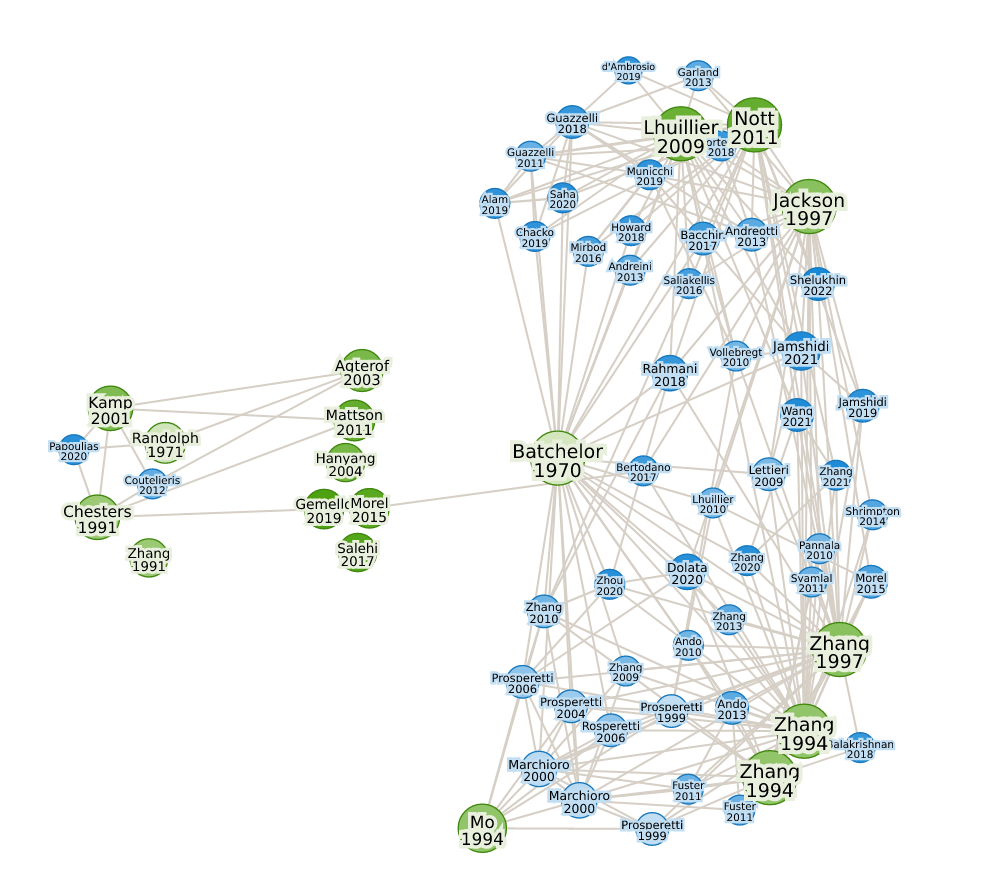
\includegraphics[width=2\textwidth]{Bib/graph70_paperGraph_network.png}};
        \draw[dashed,very thick](-2,-0.5)ellipse(1 and 2.5);
        \draw[dashed,very thick](-5,-0.5)ellipse(1.5 and 2.5);
        \draw[dashed,very thick](4,4)ellipse(2 and 1.5);
        \draw[dashed,very thick](4.5,-4)ellipse(1.5 and 2);
        \draw[dashed,very thick](4,5)node[above,very thick]{\Large$\bm{(III)}$};
        \draw[dashed,very thick](6,-5)node[right,very thick]{\Large$\bm{(II)}$};
        \draw[dashed,very thick](-6.5,2)node[above,very thick]{\Large$\bm{(I)}$};
        \draw[dashed,very thick](-1.3,1.75)node[above,very thick]{\Large$\bm{(IV)}$};
        % \draw[<->](com2.north)--(com3.south)node[midway]{Equivalent};
    \end{tikzpicture}
    \caption{Non-exhaustive cartography of the different publications on population balance models and averaged equations. The articles are represented by the name of the first author. The lines between each article mean that both articles cited each other.}
    \label{fig:carte}
\end{figure}
\ref{fig:carte} summarize the main area related to the theoretical modeling of emulsion through the averaged technics. 
The area denoted by $\bm{(I)}$ corresponds to the study dedicated to the modeling of coalescence and break up phenomenon in a suspension of droplets or bubbles.
It includes the so-called Population Balance Model (PBM) theory.
The PBM models serve to describe the evolution of the droplets size-distribution within the process. 
But also the modeling of the film drainage when two drops nearly coalesce. 
Indeed, \citet{randolph2012theory} introduced the first population balance models, at the origin it was designed  for Crystallizes. 
Then, \citet{chesters1991modelling} studied the film-drainage problem for a pair of droplets leading to coalesce kernels hence belonging to this category.
And finally, we can observe the first model of PBM including coalescence for a population of droplets \citep{KAMP20011363}.  
These PBEs often posse closure adapted to droplets or bubbles, however they are derived under the assumption of spherical solid particles since it is based on a kinetic-theory-like approach. 

The $\bm{(II)}$ and $\bm{(III)}$ area are the authors who studied the averaged equations for a mono-disperse multi-phase flow of spherical particles.
Therefore, the PBE is not involved here.
Rather they focused on closing the averaged equations theoretically. 
We consider two district formalism, the one represented here by the main article, \citet{jackson1997locally} and the other by \citet{zhang1994averaged}.
The first one makes use of volume average method and the second one of ensemble average method (those methods will be discussed in \ref{chap:daniel1}).
The interesting feature about these studies is that they both make the link between the kinetic-theory like equation while taking in account of the finite-size nature of the particles and how they are related to the continuous phase equations. 
However, this kind of averaged equations are usually derived for solid spherical particles or droplets. 
%%%%%%%%%%% I was there

To model a poly-disperse suspension of particles (either solid, bubbles or droplet) one has to links the two former theories together, that is the $\bm{(IV)}$ area. 
That is done notably by \citep{lhuillier2000bilan,morel2015mathematical,salehi2017population,gemello2018modelling}. 


The current state of the art regarding droplets suspension is incomplete.
Indeed, most of the averaged equations are derived for spherical solid particles and do not take in account of the fluid nature of the particles, such as the complex inner motion within the droplets and surface tension. 
As it will be demonstrated taking in account these properties especially impact the energy equations. 
The model the processes we woulf like to uses PBE with fluid inclusion that coalesce such as \citet{randolph2012theory}. 
Even in the case the equations governing the dispersed phase is not clearly related to the continuous phase. 
Thus, there is a clear need to derive a ``kinetic-theory'' like set of equations for fluid particle so that they can be derived with a similar methodology as PBE. 
For instance the PBE equation are derived assuming point of mass particles following ``kinetic-theory''. 

\subsection{Interaction dynamics and microstructure of dispersed two-phase flow}

Inoreder to feed PBE one need to c

\subsection{The lake of theoretical and empirical models}




\section{Ambition and objectives of this PhD.}




As the complete problem constitutes an enormous task this PhD focuses on two main aspects: 
(1) The mathematical modeling of dispersed two-phase flow, including the study of the averaged equation and the related closure problem; and (2) the numerical modeling of the PR-DNS simulation to feed those averaged equation in the context of mono-disperse buoyant emulsion. 
Although a lot of studies already exist on the topic of mathematical modeling of disperse two phase flow we demonstrate in the first chapter that there is a clear lake in the literature to take in account itermadate viscosity ratio between the droplets and continuous phase, as most of the studies focuse either on bubbles or solid particles.
Additionally, most of the averaged equations are derived for spherical solid
particles and do not take in account of the fluid nature of the particles, that  include complexe inner motion and surface tension properties, in opposition to solid particles


In this work we study only the modeling of the momentum and mechanical energy related equation-and closure terms. 
This means that we mainly focus on the mechanical subject rather than the chemical and microscale problematics involved in the problem. 
% However, note that we take in account in our theoretical and numerical studies the surface tension of droplets. 
Thus, we won't dive into the film-drainage problem and its modeling.   
Nevertheless, we still provide indispensable information regarding the ``Constrained'' or ``input'' parameters that are useful for the film drainage problem, such as the interaction behavior between droplets. 
We will not carry the Euler-Euler simulations either.
Nevertheless as we still derive the averaged equation we propose at the end of the PhD the strategy to put in place such modelisaiton including the novels models that tare developed all along this manuscript. 
At the end gives a glimpse of Euler-Euler simulation. 

\begin{figure}[h!]   
    \centering
    \begin{tikzpicture}[font=\footnotesize,very thick, scale = 0.9] 
        % \node (img0) at (-0.1\textwidth,-0.35\textwidth) {
\includegraphics[height=0.1\textwidth]{image/logo.png}};
        \node (img1) at (-0.35\textwidth,0.25\textwidth) {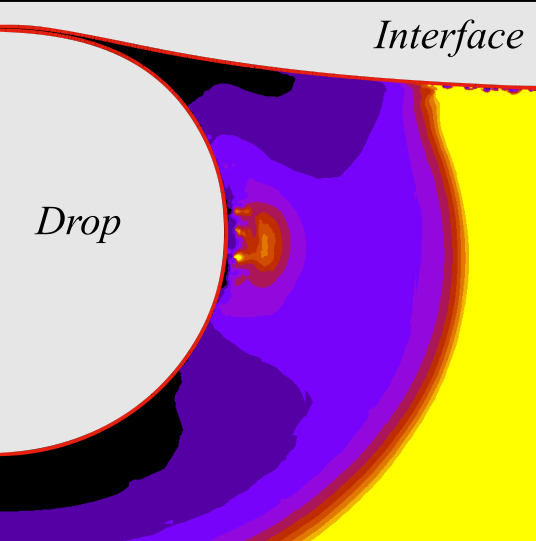
\includegraphics[height=0.25\textwidth]{image/film_drainage.png}};
        \node (img2) at (0\textwidth,0\textwidth) {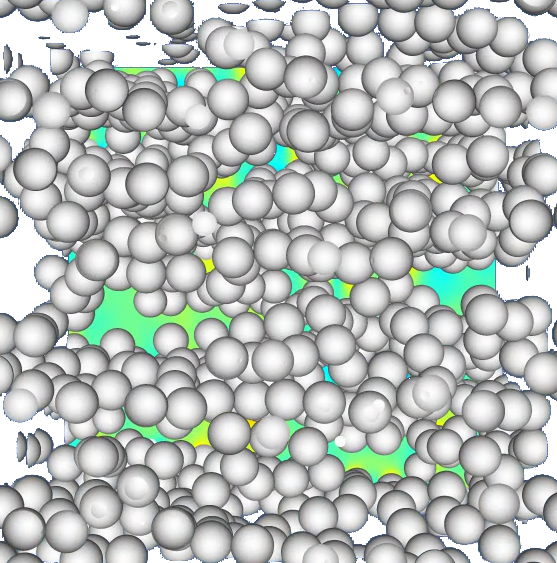
\includegraphics[height=0.25\textwidth]{image/700drop.png}};
        \node[very thick,fill=white,draw=gray] (ttx) at (0\textwidth,0.25\textwidth)
        {
        \begin{minipage}{4.4cm}
            Closure terms:
            \begin{itemize}[topsep=0pt, partopsep=0pt]
                \setlength{\itemsep}{0pt} 
                \setlength{\parskip}{0pt}
                \item \textcolor{red}{Interphase drag force}.
                \item \textcolor{red}{Velocity fluctuation}.
                \item Coalesence kernel.
                \item \ldots
            \end{itemize}
        \end{minipage}
        };
        \node[very thick,fill=white,draw=gray] (ttx2) at (0\textwidth,-0.35\textwidth)
        {
            \begin{minipage}{4.4cm}
                Constrained parameters:
                \begin{itemize}[topsep=0pt, partopsep=0pt]
                    \setlength{\itemsep}{0pt} 
                    \setlength{\parskip}{0pt}
                    \item Volume fractions. 
                    \item Phase density ratio. 
                    \item Phase viscosity ratio. 
                    \item \ldots
                    % \item Frequency of collision. 
                    % \item Interaction forces.
                \end{itemize}
            \end{minipage}
        };
        \node (img3) at (0.35\textwidth,0.25\textwidth) {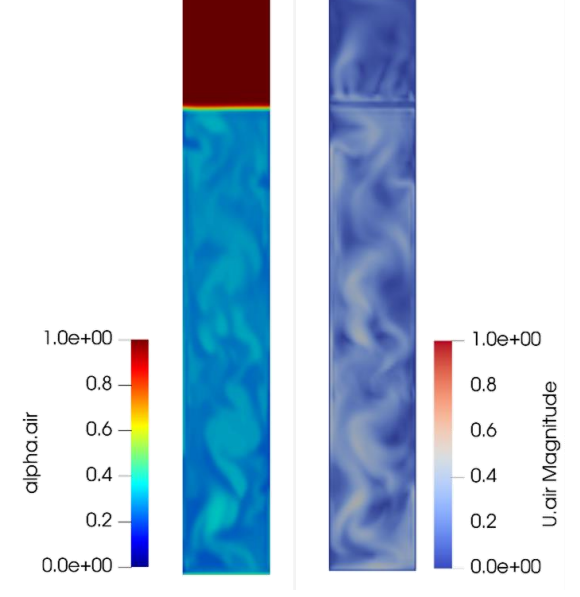
\includegraphics[height=0.25\textwidth]{image/Euler_Euler.png}};
        \node (img4) at (0.35\textwidth,-0.25\textwidth) {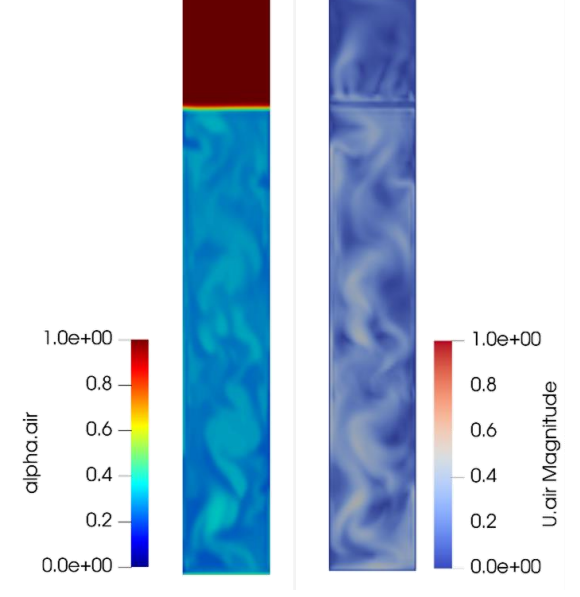
\includegraphics[height=0.25\textwidth]{image/Euler_Euler.png}};
        %                   
        %                   
        %                   
        \node[align=center] (imgB) at (-0.35\textwidth,-0.48\textwidth) {\Large \underline{Film scale}};
        \node[align=center] (imgB) at (0,-0.48\textwidth) {\Large \underline{Particles scale}};
        \node[align=center] (imgB) at (0.35\textwidth,-0.48\textwidth) {\Large \underline{Process scale}};
        %
        \node[above,text width=0.3\textwidth] (imgC) at (img1.north) {Direct Numerical Simulation (DNS).};
        \node[below,text width=0.3\textwidth] (imgD) at (img2.south) {Particles Resolve Direct Numerical Simulation (PR-DNS).};
        \node[above,text width=0.3\textwidth] (imgC) at (img3.north) {Euler-Euler simulation of the processes. };
        \node[below,text width=0.3\textwidth] (imgC) at (img4.south) {Prototype / final product};
        %
        %
        \draw[->,very thick] (img1) -- (ttx.west);
        \draw[->,very thick] (img3) -- (img4)node[midway,fill=white,draw=gray]{
        \begin{minipage}{4.4cm}
            Optimized:
            \begin{itemize}[topsep=0pt, partopsep=0pt]
                \setlength{\itemsep}{0pt} 
                \setlength{\parskip}{0pt}
                \item Geometry of process. 
                \item Inter-phase transfer.
                % \begin{itemize}[topsep=0pt, partopsep=0pt]
                %     \setlength{\itemsep}{0pt} 
                %     \setlength{\parskip}{0pt}
                %     \item Thermique
                %     \item Chemical
                % \end{itemize}
                \item \ldots
            \end{itemize}
        \end{minipage}
        };
        \draw[->,very thick] (img2.north) -- (ttx);
        \draw[->,very thick] (img2) -| (img1)node[midway,fill=white,draw=gray]{
        \begin{minipage}{4.4cm}
            Constrained parameters:
            \begin{itemize}[topsep=0pt, partopsep=0pt]
                \setlength{\itemsep}{0pt} 
                \setlength{\parskip}{0pt}
                \item \textcolor{red}{Interaction kinematic}. 
                \item Frequency of collision. 
                \item Interaction forces.
            \end{itemize}
        \end{minipage}
        };
        \draw[->,very thick] (img4) -- (ttx2);
        \draw[->,very thick] (ttx2) -- (imgD);
        %
        \draw[->,very thick] (ttx.east) -- (img3);
        \draw[red,very thick] (img2.south west) rectangle(img2.north east);
        %
        \draw[very thin, dashed] (current bounding box.north)++(-0.175\textwidth,0) -- (-0.175\textwidth,0);
        \draw[very thin, dashed] (current bounding box.south)++(-0.175\textwidth,0) -- (-0.175\textwidth,0);
        \draw[very thin, dashed] (current bounding box.north)++(0.175\textwidth,0) -- (0.175\textwidth,0);
        \draw[very thin, dashed] (current bounding box.south)++(0.175\textwidth,0) -- (0.175\textwidth,0);
    \end{tikzpicture}
    \caption{Scaling up strategy of the processes' optimization.  The text in red and the red box represents the topics treated in this PhD.}
    \label{fig:scaling_up}
\end{figure}

In \ref{fig:scaling_up} we present a diagram that summarize to whole modling strategy. 
Note, that the text and the box colored in red represent some of the topics dealt in this manuscript. 
As one can observe a lot of work is still necessary. 


\section{Outline of the manuscript}


In order to provide a consistent methodology to derive averaged equations and useful closure terms to feed the former equations we partitioned this manuscript into three main parts. 

The first part focus solely on the mathematical modeling of dispersed two phase flows, including the development of theoretical closure. 

The first Chapter of this part provides a derivation of the averaged equations governing the motion of dispersed two-phase flows with interfacial transport. 
We begin by revisiting the two-fluid formulation, as well as the distributional form of the interfacial transport equation which holds on the entire domain. 
Following this, a general Lagrangian model is introduced, which accounts for the effects of both internal and interfacial properties of the dispersed inclusions (bubbles, droplets, or particles) within a continuous phase.
We then proceed by deriving the lesser-known conservation equations for the moments of the volume and surface distribution of an arbitrary Lagrangian property.
The paper concludes by presenting a ”hybrid” set of equations, consisting of phase-averaged equations for the continuous fluid phase, complemented by an arbitrary number of moment conservation equations for the dispersed phase.
The goal of this chapter was to provide the most general approaches to derive averaged equation so that the reader obtain a wide understanding of the mathematical structure of these equations. 

In the second Chapter we expose the minimal set of equations necessary to describe emulsions made of Newtonian droplets based on the ``hybrid'' models developed in the preceding Chapter. 
In short, we expose the ensemble-averaged momentum and energy equations in the ``hybrid'' formalism for arbitrary Newtonian droplet including surface tension properties. 
Notably, this derivation allowed us to discuss the energy exchange present in a a dispersed two-phase flow. 
Additionally, we provided an explicit and general formulation for the effective stress in an emulsion. 

In the third Chapter we propose to expose a new strategy developed in this Thesis which makes the theoretical links between the closure terms and the closure problem. 
This methodology is inspired from \citet{hinch1977averaged} and generalized.
After deriving the closure problem itself we derive the closure terms for spherical droplets in stokes flow.  

Finally, in the last chapter of this part we decide to focus on the modeling of rising ellipsoidal droplets. 
We propose a set of equations that use the hybrid model to describe ellipsoidal rising droplets' droplet. 





The first parts was entirely theoretical, hence in the second part we propose to introduce DNS of rising buoyant emulsion of droplets. 
These simulations are conducted using the open source library \texttt{Basilisk C}. 

In the first chapter of this part we charaterize the particles relative position, that is termed the study of the microstructure of the emulsion. 

In the following chapter we then study the relative velocity between particles, that is the study of the kinematic of the microstructure. 

Both chapter provides useful information for the understanding of how in average pair of droplets interact together. 
Besides we introduce the nearest particle statistics in these chpater, which will proves useful for the subsequent derivations. 


The last part focus on the acctual production of the closure term, which are valid on a wide range of dimensionless parameters, in opposition to the closure presented on the part one which were often limited to stokes flow regime. 

In chpater 7 we develop a model for the drag force 
In chap 8 for the reynolds stress
In chap 9 for the particle velocity varience 